% ===========================================================================
% Section 5: Main result -- which part of the DAOD advantage is adaptation
% ===========================================================================
\section{Main Result: Which Part of the DAOD Advantage Is Adaptation}\label{sec:main}

\subsection{\texorpdfstring{\aldi}{ALDI++} versus Fine-Tuning}\label{sec:aldi-vs-ft}

\begin{table*}[t]
\centering
\caption{$\Delta(N) = {}$\aldi $-$ FT, reliable mAP$_{50:95}$, mean over seeds (95\% CI). At $N = 0$, the baseline is zero-shot.}
\label{tab:delta}
\footnotesize
\setlength{\tabcolsep}{3pt}
\begin{tabular}{@{}lccccc@{}}
\toprule
Shift & $N = 0$ & $N = 10$ & $N = 100$ & $N = 1{,}000$ & $N = 5{,}000$ \\
\midrule
lighting & \textbf{+0.009} (0.008, 0.011) & \textbf{+0.070} (0.068, 0.073) & \textbf{+0.015} (0.014, 0.017) & $-$0.011 ($-$0.012, $-$0.009) & $-$0.010 ($-$0.011, $-$0.008) \\
weather & \textbf{+0.006} (0.003, 0.007) & \textbf{+0.057} (0.050, 0.066) & \textbf{+0.014} (0.009, 0.019) & $-$0.003 ($-$0.005, $-$0.001) & \\
compound & \textbf{+0.011} (0.008, 0.014) & \textbf{+0.061} (0.054, 0.068) & \textbf{+0.016} (0.012, 0.019) & $-$0.012 ($-$0.014, $-$0.009) & \\
\bottomrule
\end{tabular}
\tabnote{Bold: an advantage that is meaningful under the rule. Weather at $N = 0$ only just passes the threshold (0.0055). At $N = 1{,}000$ the \aldi runs are the original 2,000-update runs; the results after matching are in Section~\ref{sec:matched}.}
\end{table*}

Table~\ref{tab:delta} gives $\Delta(N)$ for each shift and budget. Under the original rule, the crossover \Nx lies in the interval $(100, 1{,}000]$ in all three shifts. The \aldi curve is almost flat: from $N = 0$ to $N = 1{,}000$ it rises by only 0.003--0.010 AP, whereas the FT curve is much steeper after the overfitting region at small $N$ (Table~\ref{tab:abs}, Figs.~\ref{fig:rq5-lighting}--\ref{fig:rq5-weather}).

\begin{table}[t]
\centering
\caption{Absolute mAP (reliable, mean over seeds). DA is \aldi with the original number of updates.}
\label{tab:abs}
\footnotesize
\setlength{\tabcolsep}{3pt}
\begin{tabular}{@{}lcccccccc@{}}
\toprule
 & & \multicolumn{4}{c}{DA at $N$} & \multicolumn{2}{c}{FT at $N$} & FT \\
\cmidrule(lr){3-6}\cmidrule(lr){7-8}\cmidrule(l){9-9}
Shift & zero-shot & 0 & 10 & 100 & 1,000 & 100 & 1,000 & \begin{tabular}[b]{@{}c@{}}full pool,\\3 epochs\end{tabular} \\
\midrule
lighting & 0.244 & 0.253 & 0.253 & 0.260 & 0.262 & 0.244 & 0.273 & 0.296 \\
weather & 0.320 & 0.326 & 0.323 & 0.327 & 0.329 & 0.314 & 0.332 & 0.336 \\
compound & 0.219 & 0.230 & 0.230 & 0.239 & 0.240 & 0.223 & 0.252 & 0.257 \\
\bottomrule
\end{tabular}
\tabnote{Lighting at $N = 5{,}000$: \aldi 0.276, FT 0.286. The last column is the 3-epoch full-pool FT, the reference point for RQ5, not the 12-epoch \mAPc.}
\end{table}

\begin{figure}[t]
\centering
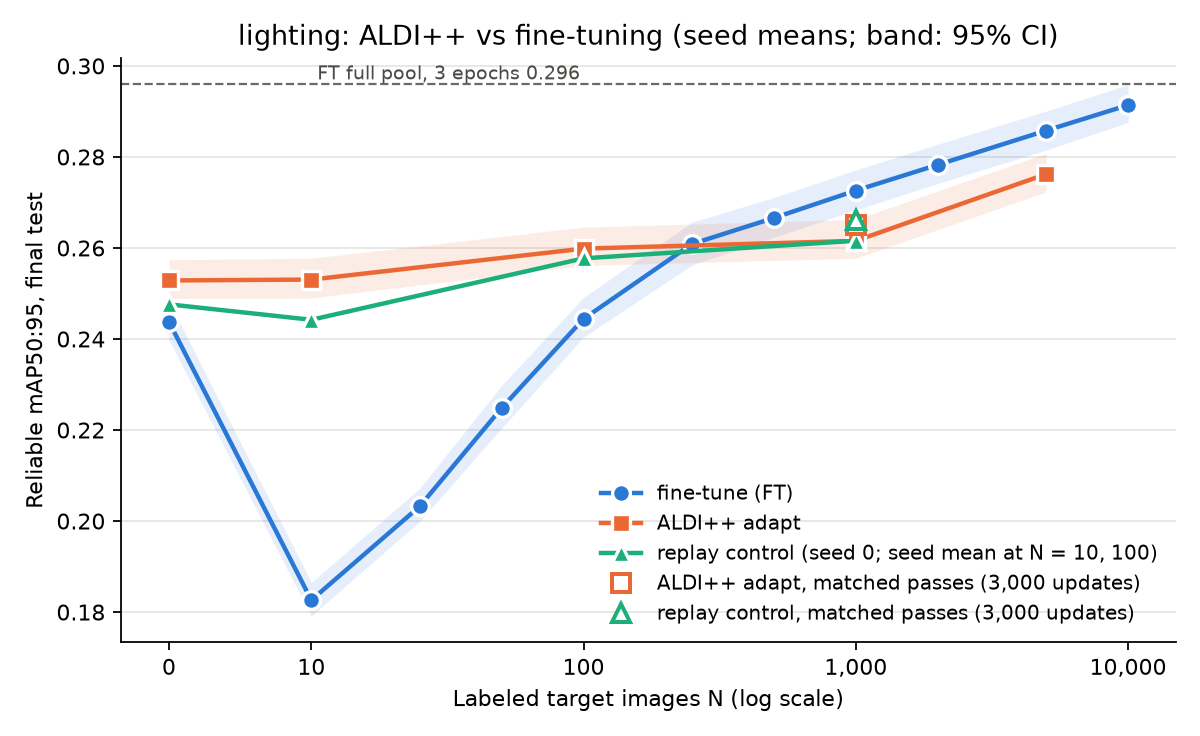
\includegraphics[width=\columnwidth]{rq5_lighting.png}
\caption{Lighting: FT, \aldi and the replay arm as a function of the budget $N$ (mean over seeds, 95\% CI bands). The open squares and triangles are the matched-passes experiment at $N = 1{,}000$ (3,000 updates).}
\label{fig:rq5-lighting}
\end{figure}

\begin{figure}[t]
\centering
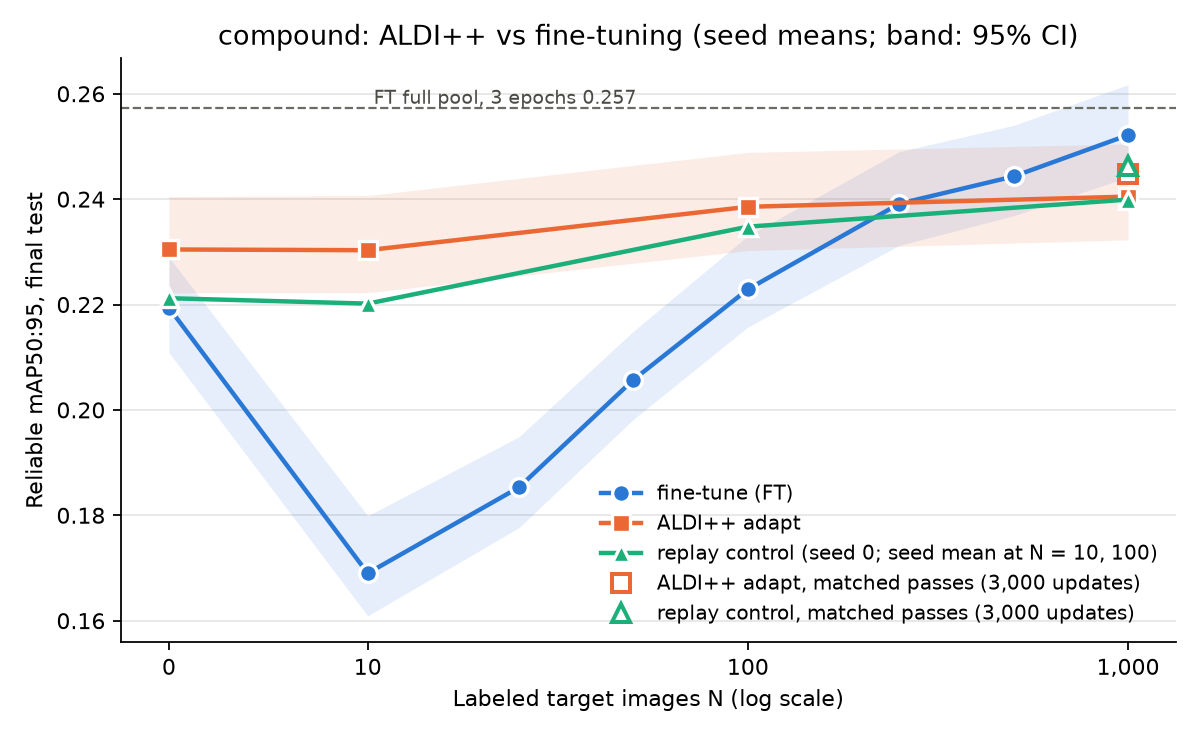
\includegraphics[width=\columnwidth]{rq5_compound.png}
\caption{Compound: same layout as Fig.~\ref{fig:rq5-lighting}.}
\label{fig:rq5-compound}
\end{figure}

\begin{figure}[t]
\centering
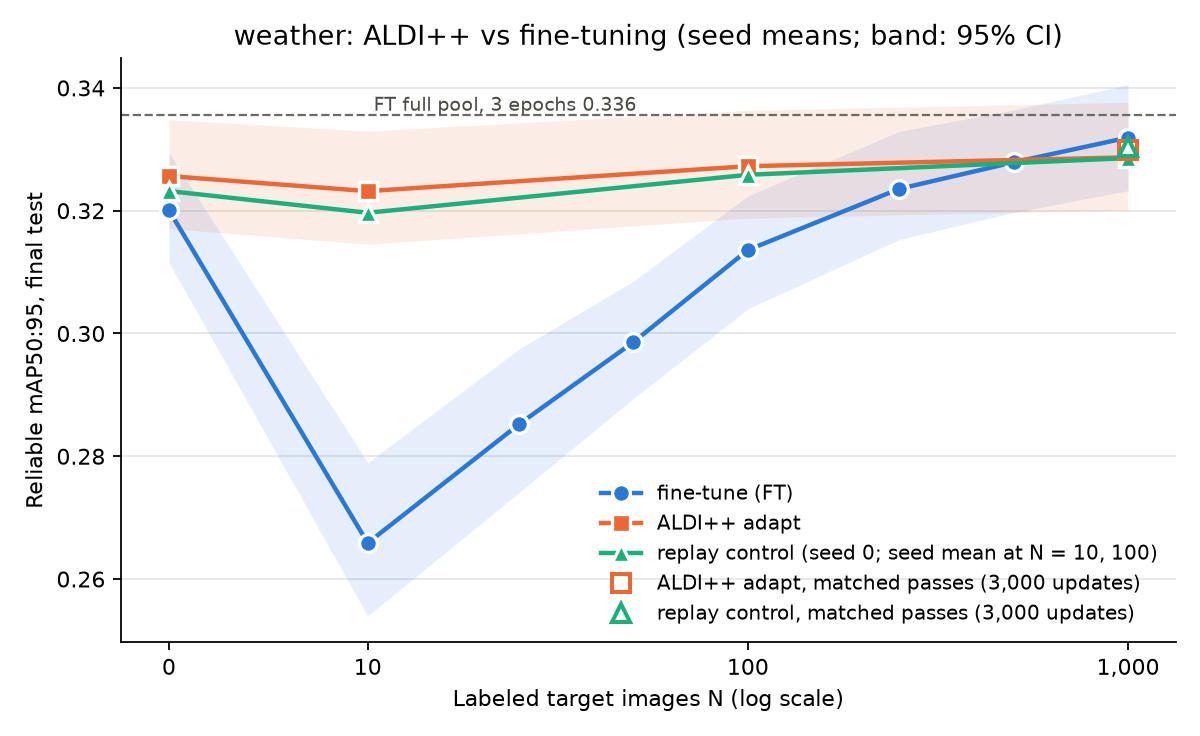
\includegraphics[width=\columnwidth]{rq5_weather.png}
\caption{Weather: same layout as Fig.~\ref{fig:rq5-lighting}. Note that the vertical-axis range is much narrower.}
\label{fig:rq5-weather}
\end{figure}

\subsection{Decomposition with the Replay Arm}\label{sec:decomp}

\begin{table}[t]
\centering
\caption{Replay share $=$ (replay $-$ FT) / (adapt $-$ FT): the part of \aldi's advantage over FT that the arm without adaptation reproduces (95\% CI).}
\label{tab:share}
\footnotesize
\setlength{\tabcolsep}{3pt}
\begin{tabular}{@{}>{\raggedright\arraybackslash}p{0.62in}>{\raggedright\arraybackslash}p{0.78in}>{\raggedright\arraybackslash}p{0.78in}>{\raggedright\arraybackslash}p{0.92in}@{}}
\toprule
$N$ & lighting & weather & compound \\
\midrule
10 (3 seeds) & \textbf{0.87} (0.85--0.90) & \textbf{0.94} (0.91--0.96) & \textbf{0.83} (0.80--0.86) \\
100 (3 seeds) & \textbf{0.86} (0.78--0.90) & \textbf{0.90} (0.81--1.04) & \textbf{0.76} (0.62--0.85) \\
1,000 (seed 0; deficit) & 1.05 (0.95--1.16) & undetermined (926/1,000) & 0.97 (0.82--1.15) \\
0 (seed 0; no labels) & 0.39 (0.28--0.45) & undetermined (287/1,000) & 0.17 ($-$0.04 to 0.35); 1/1,000 undetermined \\
\bottomrule
\end{tabular}
\tabnote{The number in parentheses after ``undetermined'' is the number of bootstrap resamples, out of 1,000, with $|\mathrm{adapt} - \mathrm{FT}| < 0.005$.}
\end{table}

\claimbox{\textbf{Main claim.} At $N = 10$ and $N = 100$, the replay arm reproduces 76--94\% of \aldi's advantage over FT in all three shifts. \aldi is genuinely ahead of FT in all six cells, every lower CI bound is above 0.5, and in no cell are more than 5\% of the bootstrap resamples undetermined. The condition recorded in advance for stating the claim is met at both budgets.\par\smallskip
Statement: \textbf{at small labeled budgets, most of the advantage of domain adaptation over fine-tuning is not adaptation.} The claim applies only to the two budgets tested ($N = 10$, $N = 100$), only to the advantage \emph{over fine-tuning}, and is not stated for $N = 0$.}

At $N = 1{,}000$, adapt $-$ FT is negative, so the share in the $N = 1{,}000$ row of Table~\ref{tab:share} says that the \emph{deficit} lies almost entirely in replay; this is not evidence for the main claim. At $N = 0$ the opposite holds: for lighting and compound, most of the gain comes from distillation, so the claim is not stated for the unlabeled case.

FT at $N \leq 50$ is below even the source model, so the same numbers read differently when the baseline is ``no fine-tuning''. Table~\ref{tab:vssource} recomputes the decomposition with the source model as the baseline.

\begin{table}[t]
\centering
\caption{Gain over the source model (mAP $-$ zero-shot). FT: mean of 3 seeds; replay and \aldi: 3 seeds at $N = 10$ and 100, seed 0 at $N = 1{,}000$ (original number of updates).}
\label{tab:vssource}
\footnotesize
\setlength{\tabcolsep}{3pt}
\begin{tabular}{@{}lrccc>{\raggedright\arraybackslash}p{1.2in}@{}}
\toprule
Shift & $N$ & FT & replay & \aldi & replay / \aldi (95\% CI) \\
\midrule
lighting & 10 & $-$0.061 & 0.000 & +0.009 & 0.05 ($-$0.09 to 0.21) \\
 & 100 & +0.001 & +0.014 & +0.016 & 0.87 (0.80--0.91) \\
 & 1,000 & +0.029 & +0.018 & +0.018 & 0.97 (0.92--1.03) \\
\addlinespace[2pt]
weather & 10 & $-$0.054 & 0.000 & +0.003 & undetermined (908/1,000) \\
 & 100 & $-$0.007 & +0.006 & +0.007 & 0.80 (0.57--1.07); 29/1,000 undetermined \\
 & 1,000 & +0.012 & +0.008 & +0.008 & 1.00 (0.86--1.24); 1/1,000 undetermined \\
\addlinespace[2pt]
compound & 10 & $-$0.050 & +0.001 & +0.011 & 0.07 ($-$0.22 to 0.29) \\
 & 100 & +0.003 & +0.015 & +0.019 & 0.80 (0.72--0.88) \\
 & 1,000 & +0.033 & +0.021 & +0.020 & 1.02 (0.92--1.12) \\
\bottomrule
\end{tabular}
\end{table}

Tables~\ref{tab:share}, \ref{tab:vssource} and~\ref{tab:cells} (the per-cell decomposition) support four conclusions:
\begin{enumerate}
\item \textbf{At $N = 10$, \aldi's large advantage over FT is damage that FT does to itself, not adaptation.} FT with 10 images and 500 updates makes the model 0.05--0.06 AP worse than the source model. Replay only has to avoid that damage to reproduce 83--94\% of the advantage. Against the source model, replay gains nothing (all CIs contain 0), and \aldi gains only +0.003 to +0.011 AP, no more than it gains with no labels at all (+0.006 to +0.011 at $N = 0$). In other words, the 10 labeled images add nothing; the small remaining gain comes from distillation.
\item \textbf{At $N = 100$, the two baselines give the same conclusion; this is the cleanest evidence.} FT is now roughly equal to the source model on lighting (+0.001) and compound (+0.003), with CIs that contain 0. On weather, FT is still 0.007 AP below the source model (CI $-0.012$ to $-0.002$), so part of the advantage here is still FT's damage. Replay reproduces 76--90\% of the advantage over FT and 80--87\% of the gain over the source model.
\item \textbf{Distillation on unlabeled images has a real but small value:} about 0.003--0.010 AP when $N \leq 10$, $\leq 0.004$ AP at $N = 100$ (on weather, the 3-seed mean is +0.001 with a CI that contains 0), and it falls to 0 at $N = 1{,}000$.
\item \textbf{The deficit at $N = 1{,}000$ is not caused by distillation.} Replay trails FT by almost the same amount, and against the source model replay equals \aldi (ratio $\approx 1$). The matched-passes experiment in Section~\ref{sec:matched} gives the same conclusion.
\end{enumerate}

\begin{table}[t]
\centering
\caption{Per-cell decomposition, seed 0 (original number of updates). The CIs reflect test-image noise only.}
\label{tab:cells}
\footnotesize
\setlength{\tabcolsep}{3pt}
\begin{tabular}{@{}lrll@{}}
\toprule
Shift & $N$ & adapt $-$ replay & replay $-$ FT \\
\midrule
lighting & 0 & +0.006 & +0.004 \\
 & 10 & +0.009 & +0.062 \\
 & 100 & +0.002 & +0.012 \\
 & 1,000 & 0.000 (CI contains 0) & $-$0.010 \\
\addlinespace[2pt]
weather & 0 & +0.003 & +0.003 \\
 & 10 & +0.004 & +0.064 \\
 & 100 & +0.003 & +0.016 \\
 & 1,000 & 0.000 (CI contains 0) & $-$0.003 \\
\addlinespace[2pt]
compound & 0 & +0.009 & +0.002 (CI contains 0) \\
 & 10 & +0.010 & +0.046 \\
 & 100 & +0.004 & +0.013 \\
 & 1,000 & 0.000 (CI contains 0) & $-$0.012 \\
\bottomrule
\end{tabular}
\tabnote{At $N = 0$, ``replay'' is the source model trained further on source images with strong augmentation and EMA, so replay $-$ FT here is replay $-$ zero-shot.}
\end{table}

\subsection{Matched-Passes Experiment at \texorpdfstring{$N = 1{,}000$}{N = 1,000}}\label{sec:matched}

In the original grid, at $N = 1{,}000$, FT runs 1,500 updates with 2 labeled target images per step (about 3,000 passes), while \aldi and replay run 2,000 updates with 1 labeled target image per step (about 2,000 passes). \aldi's deficit is therefore confounded with the difference in the amount of labeled training. The matched-passes experiment reruns \aldi and replay with 3,000 updates and 3 seeds. The reading rule, recorded before scoring: ``FT leads from $N = 1{,}000$'' stands when the difference is $\leq -0.005$ and the upper CI bound is below 0; otherwise it is withdrawn. The text of the rule does not say whether it applies to the three shifts pooled or to each shift separately; here it is applied per shift, and this way of applying it was recorded after scoring.

\begin{table*}[t]
\centering
\caption{$N = 1{,}000$ with matched labeled target-image passes (3,000 updates, 3 seeds; 95\% CI).}
\label{tab:matched}
\footnotesize
\setlength{\tabcolsep}{3pt}
\begin{tabular}{@{}lcccc>{\raggedright\arraybackslash}p{1.2in}@{}}
\toprule
Shift & \begin{tabular}[b]{@{}c@{}}original\\\aldi $-$ FT\end{tabular} & \begin{tabular}[b]{@{}c@{}}matched\\\aldi $-$ FT\end{tabular} & \begin{tabular}[b]{@{}c@{}}matched\\replay $-$ FT\end{tabular} & \begin{tabular}[b]{@{}c@{}}\aldi $-$ replay\\(matched)\end{tabular} & Verdict under the rule \\
\midrule
lighting & $-$0.0111 & $-$0.0076 & $-$0.0064 & $-$0.0012 & ``FT leads'' stands \\
 & & ($-$0.0091, $-$0.0058) & ($-$0.0077, $-$0.0049) & ($-$0.0021, $-$0.0002) & \\
\addlinespace[2pt]
weather & $-$0.0032 & $-$0.0021 & $-$0.0015 & $-$0.0005 & withdrawn: no meaningful difference \\
 & & ($-$0.0038, +0.0002) & ($-$0.0034, +0.0006) & ($-$0.0022, +0.0011) & \\
\addlinespace[2pt]
compound & $-$0.0117 & $-$0.0074 & $-$0.0058 & $-$0.0016 & ``FT leads'' stands \\
 & & ($-$0.0097, $-$0.0047) & ($-$0.0082, $-$0.0035) & ($-$0.0035, +0.0007) & \\
\bottomrule
\end{tabular}
\end{table*}

\begin{itemize}
\item The extra 1,000 updates (Table~\ref{tab:matched}) give \aldi +0.0034 / +0.0012 / +0.0043 AP (lighting / weather / compound), closing about a third of the gap (31\% / 36\% / 36\%), but they do not eliminate it on lighting and compound.
\item \textbf{Distillation contributes nothing to reliable mAP at $N = 1{,}000$.} After matching, \aldi is level with or slightly below replay; on lighting the CI of the difference does not contain 0. Per class, the changes offset each other: car gains +0.003 (lighting) and +0.002 (compound), while traffic light and traffic sign on lighting drop by 0.004 and 0.005.
\item Against the source model, replay reproduces all of \aldi's gain after matching: ratios of 1.06 (1.01--1.10) / 1.05 (0.89--1.26) / 1.06 (0.98--1.15).
\item The crossover \Nx under the original rule is unchanged, $(100, 1{,}000]$ in all three shifts. On weather it says only that \aldi's advantage disappears, not that FT pulls ahead.
\item \textbf{Limit of the matching:} it matches the number of labeled image passes that the \emph{student} sees, but the model that is scored is the EMA teacher. After 3,000 updates the source-model initialization still carries a weight of $0.9996^{3000} \approx 0.30$ in the teacher (0.45 after 2,000 updates). This lag is an alternative explanation for the remaining deficit.
\end{itemize}

\subsection{Equivalent Labeled Budget}\label{sec:neq}

\begin{table}[t]
\centering
\caption{\Neq: the number of images FT needs to reach the same mAP as \aldi (original number of updates; 95\% CI).}
\label{tab:neq}
\footnotesize
\setlength{\tabcolsep}{3pt}
\begin{tabular}{@{}lccccc@{}}
\toprule
 & \multicolumn{5}{c}{DA} \\
\cmidrule(l){2-6}
Shift & $N = 0$ & $N = 10$ & $N = 100$ & $N = 1{,}000$ & $N = 5{,}000$ \\
\midrule
lighting & 160 & 162 & 236 & 272 & 1,556 \\
 & (142--184) & (145--183) & (215--287) & (235--344) & (1,343--1,894) \\
\addlinespace[2pt]
weather & 349 & 242 & 451 & 575 & \\
 & (240--511) & (184--379) & (313--672) & (413--834) & \\
\addlinespace[2pt]
compound & 153 & 152 & 242 & 300 & \\
 & (123--182) & (121--180) & (209--332) & (233--410) & \\
\bottomrule
\end{tabular}
\end{table}

\begin{itemize}
\item Unlabeled \aldi (unsupervised domain adaptation, UDA) is worth about \textbf{150--350 labeled images} when FT is used with this schedule (Table~\ref{tab:neq}).
\item \aldi with 10 labeled images is no better than unlabeled \aldi: those 10 images add almost nothing.
\item With the original number of updates, \aldi with 1,000 labeled images is equivalent to FT with only 270--575 images. This figure is confounded with the difference in the number of labeled image passes and is not recomputed for the matched-passes experiment; on weather, no meaningful difference remains after matching, so the figure of 575 is not to be read as \aldi losing to FT.
\end{itemize}

\subsection{Weather: The Third Replication of the Decomposition}\label{sec:weather-rep}

The weather shift leaves very little to recover (Section~\ref{sec:drop}), so its thresholds can hardly be measured. The decomposition, however, needs no recovery denominator, and weather shows the same pattern as the other two shifts: a replay share of 0.94 at $N = 10$ and 0.90 at $N = 100$, with lower CI bounds above 0.5; distillation contributes only +0.001 AP at $N = 100$ (3-seed mean, CI contains 0); and at $N = 1{,}000$, after matching, neither \aldi nor replay differs meaningfully from FT. Every weather $\Delta$ except the one at $N = 10$ is small in absolute AP ($|\Delta| \leq 0.014$). The role of weather in this paper is therefore that of the third replication of the decomposition, not a third threshold measurement.
